\chapter{Related Works}

Your related works, and your purpose and contribution which must be different as below.

\section{Mhd Zulfikar Akram Nasution/1164081}
\subsection{Teori}
\begin{enumerate}
\item Binary Classification atau diartikan kedalam bahasa indonesia yaitu Klasifikasi Biner adalah tugas dalam mengklarifikasikan elemen-elemen dari himpunan yang diberikan kedalam dua kelompok berdasarkan aturan klarifikasi. Pada ummnya klarifikasi biner akan jatuh ke dalam domain Supervised Learning dan dimana kasus khusus hanya memiliki dua kelas.
\begin{itemize}
\item  Contoh Binary Classification pada gambar 2.1
\end{itemize}
\begin{figure}[ht]
\centering
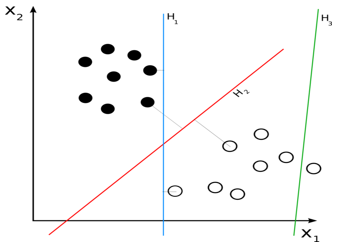
\includegraphics[scale=0.9]{figures/zulfikar/1.png}
\caption{Binary Classification}
\end{figure}

\item Supervised Learning, Unsupervised Learning, dan Clustering
\begin{itemize}
\item Supervised Learning
\end{itemize}
\par
Supervised learning adalah tugas pembelajaran mesin untuk mempelajari suatu fungsi yang memetakan input ke output berdasarkan contoh pasangan input-output. Ini menyimpulkan fungsi dari data pelatihan berlabel yang terdiri dari serangkaian contoh pelatihan. Dalam pembelajaran yang diawasi, setiap contoh adalah pasangan yang terdiri dari objek input (biasanya vektor) dan nilai output yang diinginkan (juga disebut sinyal pengawas). Contoh pada gambar 2.2
\begin{figure}[ht]
\centering
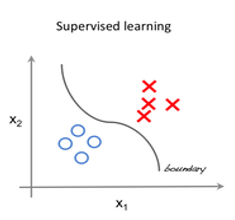
\includegraphics[scale=0.9]{figures/zulfikar/2.png}
\caption{Supervised Learning}
\end{figure}

\begin{itemize}
\item Unsupervised Learning
\end{itemize}
\par
Unsupervised Learning merupakan sebuah data yang belum ditentukan variabelnya jadi hanya berupa data saja. Dalam sebuah kasus Unsupervised Learning adalah aggap saja anda belum pernah membeli buku sama sekali dan pada suatu hari anda telah membeli buku dengan sangat banyak dalam kategori yang berbeda. Sehingga buku tersebut belum di kategorikan dan hanya berupa data buku saja. Coontoh seperti pada gambar 2.3
\begin{figure}[ht]
\centering
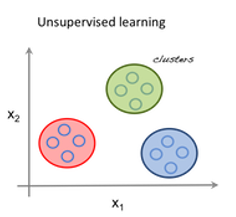
\includegraphics[scale=0.9]{figures/zulfikar/3.png}
\caption{Unsupervised Learning}
\end{figure}

\begin{itemize}
\item Clustering
\end{itemize}
\par
 Classtering merupakan sebuah proses untuk mengklasifikasikan sebuah data dalam satu parameter. Dalam kasus ini dapat dijelaskan ada beberapa orang yang memiliki kekuatan tubuh yang sehat dan kekuatan tubuh yang lemah. Parameter bagi orang yang memiliki tubuh yang kuat adalah orang yang terlihat bugar dan sehat maka dengan orang yang memiliki parameter adalah orang yang memiliki kekuatan tubuh yang kuat dan untuk kekuatan tubuh yang lemah adalah sebaliknya. Contoh seperti pada gambar 2.4
\begin{figure}[ht]
\centering
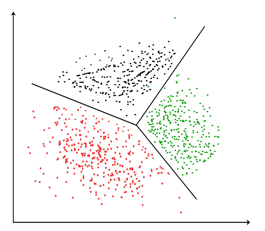
\includegraphics[scale=0.9]{figures/zulfikar/4.png}
\caption{Clustering}
\end{figure}

\item Evaluasi dan Akurasi
\par
 Evaluasi adalah tentang  bagaimana kita dapat mengevaluasi seberapa baik model bekerja dengan mengukur akurasinya. Dan akurasi akan didefinisikan sebagai persentase kasus yang diklasifikasikan dengan benar. Kita dapat menganalisis kesalahan yang dibuat oleh model, atau tingkat kebingungannya, menggunakan matriks kebingungan. Matriks kebingungan mengacu pada kebingungan dalam model, tetapi matriks kebingungan ini bisa menjadi sedikit sulit untuk dipahami ketika mereka menjadi sangat besar.

\item Cara Membuat dan Membaca Confusion Matrix
\begin{itemize}
\item Tentukan pokok permasalahan dan atributnya
\item Buat Decicion Tree
\item Buat Data Testing
\item Mencari nilai variabelnya misal a,b,c, dan d
\item Mencari nilai recall, percision, accuracy, dan error rate
\end{itemize}
\par contoh confusion matrix
	\begin{verbatim}
		Recall = 3/(1+3) = 0,75
		Percision = 3/(1+3 = 0,75
		Accuracy = (5+3)/(5+1+1+3) = 0,8
		Error Rate = (1+1)/(5+1+1+3) 0,2
	\end{verbatim}

\item Cara Kerja K-Fold Cross Validation
	\begin{itemize}
		\item Total instance dibagi menjadi N bagian.
		\item Fold yang pertama adalah bagian pertama menjadii testing data dan sisanya menjadi training data.
		\item Hitung akurasi berdasarkan porsi data tersebut dengan menggunakan persamaan.
		\item Fold yang ke dua adalah bagian ke dua menjadi testing data dan sisanya training data. 
		\item Hitung akurasi berdasarkan porsi data tersebut.
		\item Lakukan step secara berulang hingga habis mencapai fold ke-K.
		\item Terakhir hitung rata-rata akurasi K buah.
	\end{itemize}
\par
Berikut ilustrasi K-Fold Cross Validation seperti pada gambar 2.5
\begin{figure}[ht]
\centering
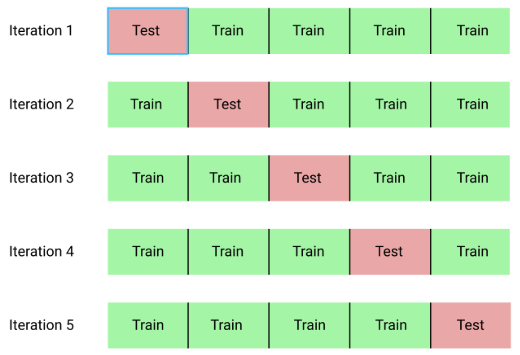
\includegraphics[scale=0.9]{figures/zulfikar/5.png}
\caption{K-Fold Cross Validation}
\end{figure}

\item Decision Tree
\par 
Decision Tree adalah sebuah metode pembelajaran yang digunakan untuk melakukan klarifikasi dan regresi. Decision Tree digunakan untuk membuat sebuah model yang dapat memprediksi sebuah nilai variabel target dengan cara mempelajari aturan keputusan dari fitur data. Contohnya seperti pada gambar 2.6 
\begin{figure}[ht]
\centering
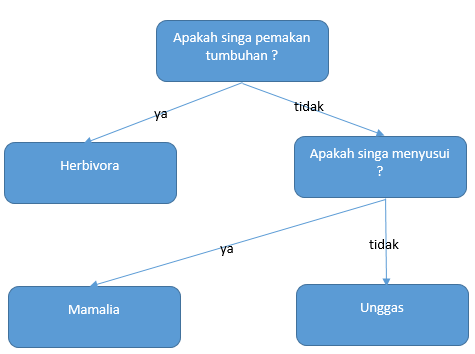
\includegraphics[scale=0.9]{figures/zulfikar/6.png}
\caption{Decision Tree}
\end{figure}

\item Gain dan Entropi
\begin{itemize}
\item Gain adalah pengurangan yang diharapkan dalam enthropy. Dalam mechine learning, gain dapat digunakan untuk menentukan sebuah urutan atribut atau memperkecil atribut yang telah dipilih. Urutan ini akan membentuk decision tree. atribut gain dipilih yang paling besar.
\item  Entropi adalah ukuran ketidakpastian sebuah variabel acak sehingga dapat di artikan entropi adalah ukuran ketidakpastian dari sebuah atribut.
\end{itemize}
\par Contoh seperti pada gambar 2.7
\begin{figure}[ht]
\centering
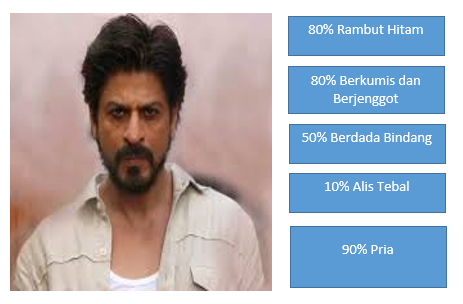
\includegraphics[scale=0.9]{figures/zulfikar/7.png}
\caption{Gain dan Entropi}
\end{figure}
\end{enumerate}


\section{Same Topics}
Cite every latest journal with same topic
\subsection{Topic 1}
cite for first topic

\subsection{Topic 2}
if you have two topics you can include here to


\section{Same Method}
write and cite latest journal with same method

\subsection{Method 1}
cite and paraphrase method 1

\subsection{Method 2}
cite and paraphrase method 2 if you have more method please add new subsection.

 